\textit{Git} es un sistema de control de versiones que permite al desarrollador crear múltiples ramas de desarrollo, sincronizar su trabajo con otros desarrolladores, revertir cambios realizados en el código y mantener una versión ordenada de un proyecto. Usar este tipo de herramientas para el desarrollo de proyectos en Vivado Desing Suite resulta ser muy útil, ya que permite trabajar de manera colaborativa y llevar registro de las versiones del hardware diseñado. En este apéndice se resumen todos los consejos y etapas para llevar a cabo el control de versiones de un proyecto Vivado. La clave del método a describir consiste subir al repositorio solo los archivos principales del proyecto, dejando fuera cualquier otro archivo proveniente de etapas de síntesis, implementación o archivos generados automáticamente por Vivado. Para llevar a cabo el control de versiones se hace uso de \textit{git} junto con la plataforma en línea \textit{Github.com}.

Antes de comenzar, se debe contar con los siguientes requisitos:
\begin{itemize}
	\item Nociones básicas de \textit{git}.
	\item Una cuenta en \textit{Github.com}.
	\item El software de control de versiones \textit{git} instalado en el computador y habilitado para ser operado mediante un terminal de comandos.
	\item Tener instalado Vivado Design Suite (La versión utilizada en este tutorial corresponde a la versión 2019.1).
\end{itemize}

\section{Creación de un repositorio Git}

	Para comenzar, se debe iniciar sesión en \textit{Github.com} y hacer clic en el botón verde  ``New'' ubicado en la esquina superior izquierda, como se ilustra en la Figura \ref{fig:git1}.
	
	\begin{figure}[ht]
		\centering
		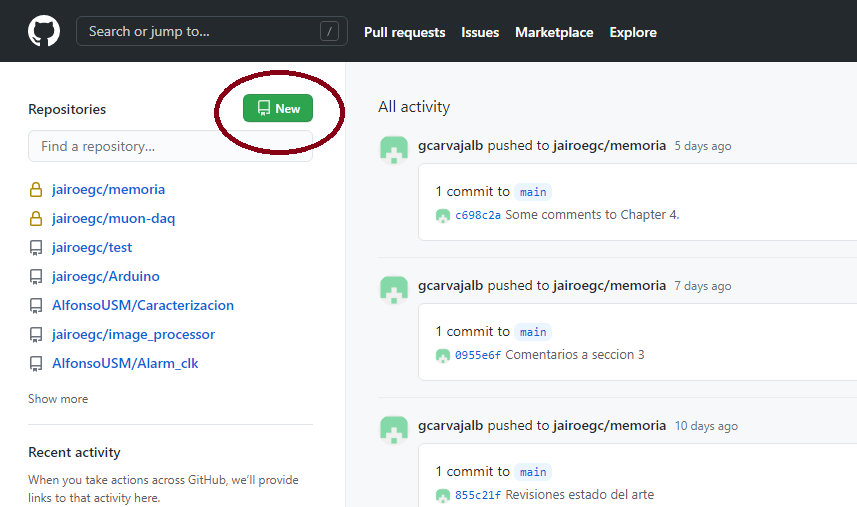
\includegraphics[scale=0.6]{git1.png}
		\caption{Botón ``New'' para la creación de un nuevo repositorio remoto en \textit{Github.com}.}
		\label{fig:git1}
	\end{figure}
	
	Se debe elegir el nombre del repositorio y configurar lo esencial. Se recomienda crear un proyecto en blanco, sin archivo \textit{readme} o \textit{.gitignore}, ya que serán subidos al repositorio de manera remota durante el primer \textit{commit}.

\section{Clonación de un repositorio Git}

	Desde la interfaz web del repositorio de Github.com debe buscarse el botón verde llamado ``Code'' (ubicado en la esquina superior derecha) y copiar en el portapapeles la \textit{URL} disponible para clonar el repositorio mediante HTTPS (Hypertext Transfer Protocol Secure), como se ilustra en la Figura \ref{fig:git2}.
	
	\begin{figure}[ht]
		\centering
		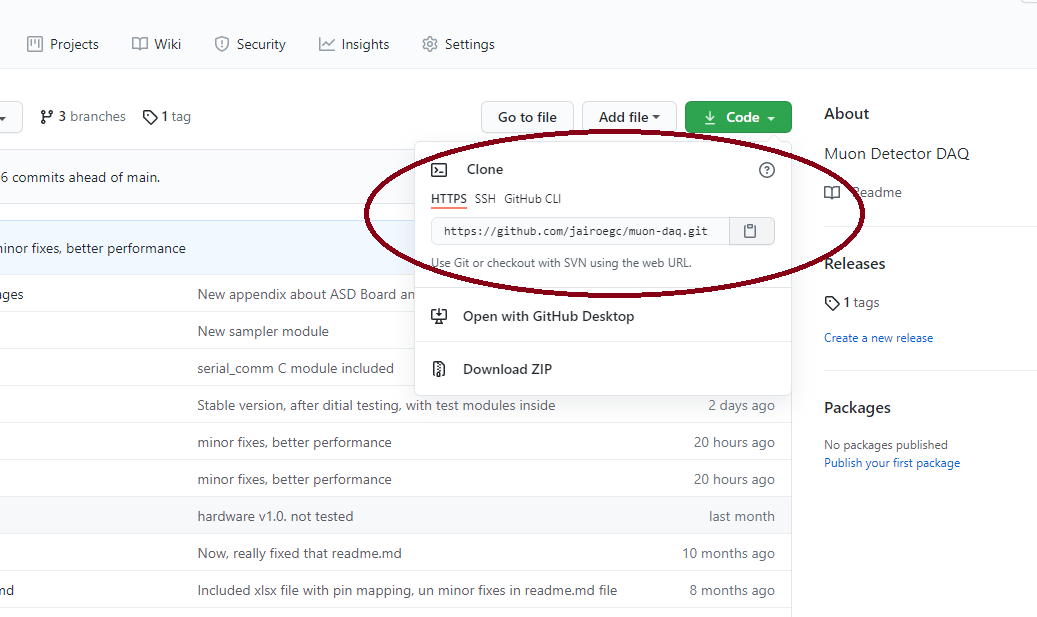
\includegraphics[scale=0.5]{git2.png}
		\caption{Botón ``Code'' para acceder al enlace de clonación del repositorio.}
		\label{fig:git2}
	\end{figure}
	
	Si aún no se tiene instalado \textit{git} en el computador, se debe proceder a su instalación vía consola o mediante descarga directa. Luego, se debe acceder o crear una carpeta para guardar el repositorio Vivado, abrir en ella una consola de comandos y escribir lo siguiente, sustituyendo \textit{your-git-url} con el enlace copiado en el portapapeles:

\begin{lstlisting}[language=bash]
$ git clone your-git-url
\end{lstlisting}


\section{Creación de los archivos y carpetas iniciales}

	Para crear los primeros archivos del repositorio se debe acceder a la carpeta escogida y crear 5 nuevas carpetas en su interior llamadas \textit{ip}, \textit{src},  \textit{sim}, \textit{xdc} y \textit{wd}.
	
	\begin{itemize}
		\item \textit{ip}: Esta carpeta incluirá los archivos asociados a IP Cores.
		\item \textit{src}: Esta carpeta es la indicada para guardar los archivos de código HDL.
		\item \textit{sim}: Carpeta para almacenar \textit{testbenchs}.
		\item \textit{xdc}: Carpeta destinada a guardar archivos XDC para \textit{constraints} y declaraciones de puertos.
		\item \textit{wd}: Esta carpeta es la indicada para guardar los archivos generados automáticamente por Vivado durante las etapas de síntesis e implementación. Esta carpeta no debe ser incluida en los \textit{commits} de \textit{git}, ya que contiene precisamente la información que no requiere seguimiento en el repositorio.	
	\end{itemize}
	
	Luego, se puede crear un archivo \textit{README.md} y uno \textit{.gitinit} en la carpeta principal. El archivo \textit{README.md} es relevante para explicar el contenido del repositorio y debe ser escrito en lenguaje \textit{Markdown}. En el archivo \textit{.gitinit} se deben incluir todos los formatos de archivo que no quieran ser subidos al repositorio, como lo son los archivos creados automáticamente por el sistema o la carpeta \textit{wd} mencionada anteriormente. Se sugiere agregar las siguientes lineas en este archivo \textit{.gitinit}:

\begin{lstlisting}[language=bash, frame=single]
wd/
.Xil/
\end{lstlisting}

\section{Preparación del proyecto Vivado}
	Antes que todo, se debe crear un proyecto Vivado y guardarlo en la carpeta \textit{wd} anteriormente creada. Si el proyecto ya existía, entonces basta con trasladar el proyecto completo y guardarlo al interior de la carpeta \textit{wd}. Luego de ello, se deben copiar o crear los archivos fuente del diseño en HDL, los archivos de simulación y los \textit{constraints} en sus respectivas carpetas.
	
	Si el diseño de hardware utiliza IP Cores, hay que asegurarse de habilitar la opción de \textit{IP Core Containers} en Vivado. Esta opción se encuentra en el menú \textit{Tools$>$ Settings$> $Project Settings$>$ IP$>$ Core Containers: Use Core Containers for IP} ilustrado en la Figura \ref{fig:viv1}, lo que facilita el control de versiones creando un solo archivo \textit{.xcix} que contiene al IP Core en su totalidad. Si Vivado pregunta por convertir el IP Core actual a un \textit{container}, dar clic en \textit{OK} y mover los \textit{containters} a la carpeta \textit{ip} correspondiente en el repositorio.
	
	\begin{figure}[ht]
		\centering
		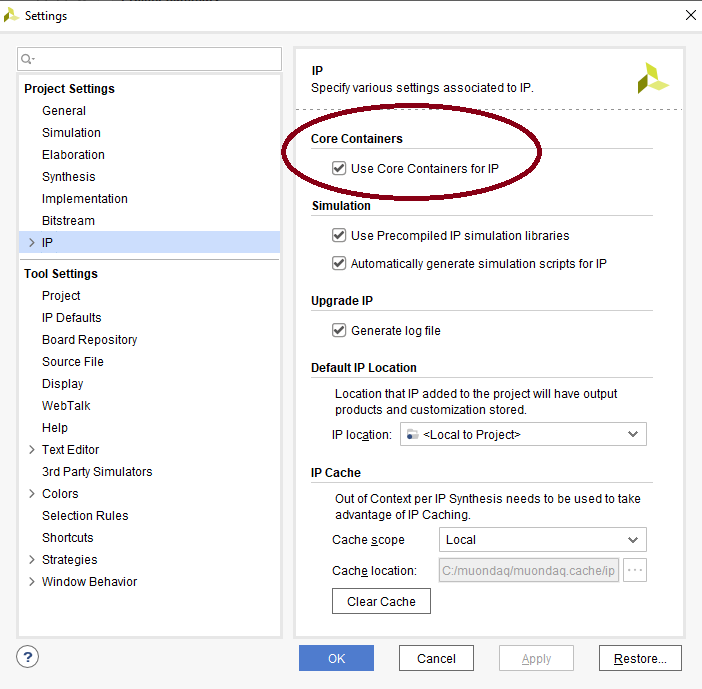
\includegraphics[scale=0.5]{viv1.png}
		\caption{Menú de configuración para la habilitación de IP Containers en Vivado.}
		\label{fig:viv1}
	\end{figure}
	
	Finalmente, se deben importar los archivos contenidos en las carpetas \textit{src, sim, xdc} e \textit{ip} al proyecto de descripción de hardware en la vista \textit{Project Manager} de Vivado.

\section{Exportar script Tcl}

	Desde la interfaz de Vivado se debe exportar el archivo \textit{Tcl} (Tool Command Language) asociado al proyecto Vivado accediendo a \textit{File$>$ Project$>$ Write Tcl} ilustrado en la Figura \ref{fig:viv2} y guardándolo con el nombre \textit{build.tcl} en la carpeta principal de repositorio, no en las subcarpetas creadas. Se debe tener encuentra que el proceso de exportación y edición del archivo Tcl debe realizarse cada vez que se crea o elimina un nuevo archivo fuente del proyecto. En caso de no realizar la exportación, el script no generará el proyecto completo y habrá que importar los archivos fuente de manera manual.
	
	\begin{figure}[ht]
		\centering
		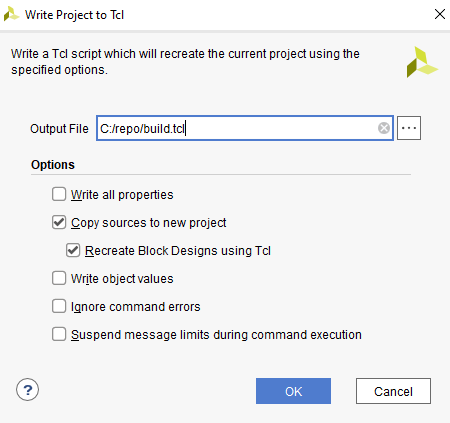
\includegraphics[scale=0.6]{viv2.png}
		\caption{Ventana de Vivado para la exportación de un script Tcl.}
		\label{fig:viv2}
	\end{figure}

\section{Editar script Tcl}
	Un paso importante en este proceso de control de versiones es la edición del archivo Tcl, para que así se generen automáticamente los archivos de Vivado en la carpeta \textit{wd}. Para lograrlo, se debe abrir el archivo \textit{build.tcl} en un editor de texto y buscar los siguientes comandos:

\begin{lstlisting}[language=bash, frame=single, basicstyle=\small]
	
# Set the reference directory for source file relative paths 
#(by default the value is script directory path)
set origin_dir "."

# Set the directory path for the original project from where
#this script was exported
set orig_proj_dir "path-to-the-actual-vivado-project"
	
# Create project
create_project ${_xil_proj_name_} ./${_xil_proj_name_} 
	-part part-of-your-fpga

\end{lstlisting}

	Una vez ubicados, se deben reemplazar por los siguientes comandos:
	
\begin{lstlisting}[language=bash, frame=single, basicstyle=\small]
	
# Set the reference directory for source file relative paths 
#(by default the value is script directory path)
set origin_dir [file dirname [info script]]

# Set the directory path for the original project from where 
#this script was exported
set orig_proj_dir "[file normalize "$origin_dir/wd/"]"

# Create project
create_project ${_xil_proj_name_} $orig_proj_dir/${_xil_proj_name_} 
	-part part-of-your-fpga

\end{lstlisting}


\section{Confirmar y subir los archivos al repositorio remoto}

	En este punto todo se encuentra listo para realizar el primer \textit{commit} en \textit{git} y comenzar el control de versiones del proyecto Vivado mediante el siguiente comando en consola:
	
\begin{lstlisting}[language=bash, frame=single]
$ git add .
$ git commit -m "First commit."
$ git push

\end{lstlisting}

	Luego de ejecutar los comandos en consola, el control de versiones se encuentra correctamente configurado y es seguro eliminar el proyecto Vivado de otras ubicaciones fuera del repositorio, ya que el proyecto puede ser reconstruido completamente al ejecutar el script \textit{ build.tcl} desde la consola Tcl de Vivado.